\documentclass[12pt]{beamer}
\usepackage{algorithm2e} %pseudocodigos
\usepackage{algorithmic} %pseudocodigos
\usepackage{float}
\usetheme{Berkeley}



\usepackage{graphicx}
\graphicspath{{imagens/}}
\usepackage{booktabs}
\usepackage[english]{babel}



\logo{\includegraphics[height=1cm]{example-image-c}}
\title[XXXX]{Uma nova heur\'istica para o "Single-Picker-Routing-Problem" com restri\c{c}\~oes pr\'aticas de carregamento}



\author{Alexandre Checoli Choueiri}
\institute[AI]
{UFPR  \\ % Your institution for the title page
	\medskip
	\textit{alexandrechecoli@gmail.com} % Your email address
	
}
\date{\today}

\begin{document}
	
	\begin{frame} 
		\titlepage % Print the title page as the first slide	
	\end{frame}
	
	\begin{frame}{Sum\'ario}
		\tableofcontents
	\end{frame}
	
	
	%   PRESENTATION SLIDES
	
\section{Motiva\c{c}\~ao} %
%------------------------------------------------


\section{Descri\c{c}\~ao do problema} %
\section{Heur\'istica de corre\c{c}\~ao de rotas} %
\section{Heur\'istica de Empacotamento} %
\section{Heur\'istica de Escoamento de Pontos (H.E.P)} %
\section{Resultados} %






\begin{frame}{Descri\c{c}\~ao do problema}
	O Problema do Caixeiro Viajante (PCV) trata da
	ordena\c{c}\~ao/sequenciamento de um dado conjunto de pontos de
	tal forma que um caminho passando por todos os pontos, uma
	\'unica vez em cada ponto, e voltando ao ponto inicial seja
	m\'inimo.
\begin{figure}
		
		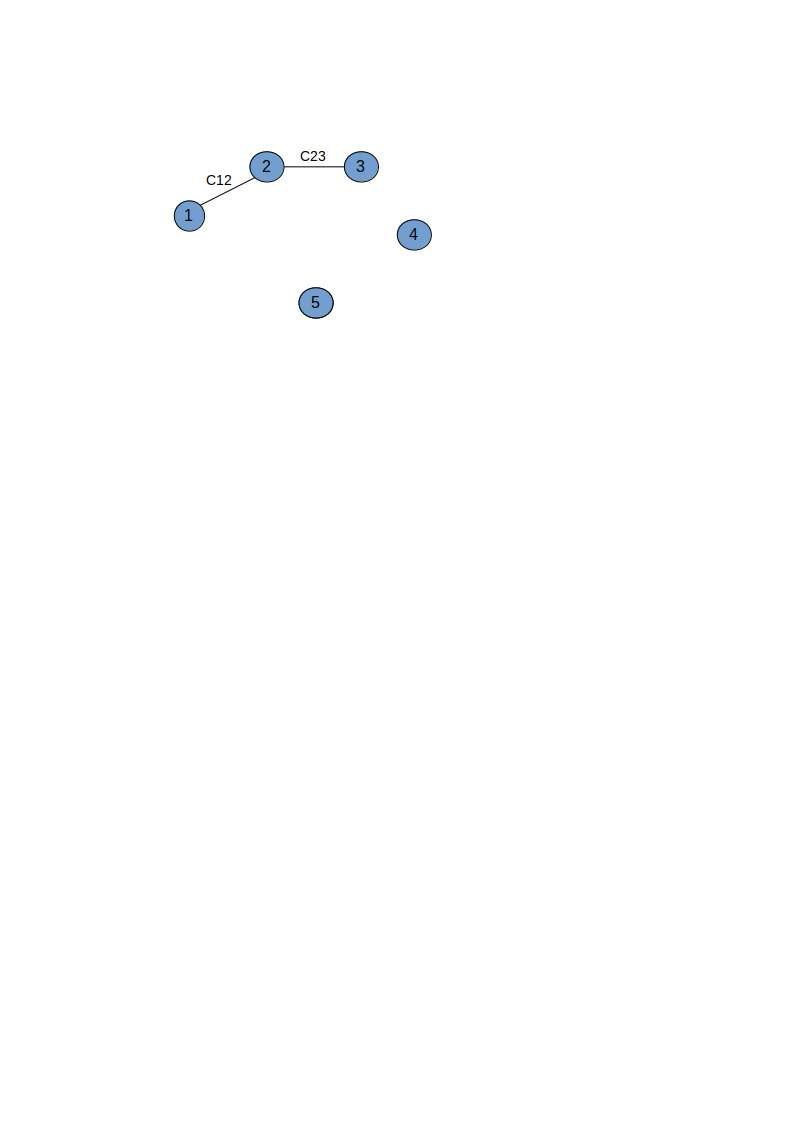
\includegraphics[width=1\linewidth]{pontos_2}
		\caption{}
\end{figure}
	
\end{frame}


	
	
	
	
	
	
\end{document} 